\chapter{Búsqueda binaria}

\section{Planetas}
Tienes un conjunto de planetas y te dan las posiciones de estos planetas, quieres colocar un metiorito en cualquier lugar entre los planetas, el meteorito debe quedarse en su lugar y no ser atraido por la fuerza gravitacional de los planetas. 
Sabemos de física básica que la sumatoria de todas las fuerzas debe ser igual con cero. Sabemos que:
\begin{itemize}
    \item $F_{1} = F_{2}$ esta en equilibrio el sitema
    \item $F_{1} > F_{2}$
    \item $F_{1} < F_{2}$
\end{itemize}

Tenemos como información la siguiente fórmula:
\[
    \frac{1}{|X_{i} - M|}    
\]

Ejemplo:
\begin{figure}[H]
    \begin{center}
    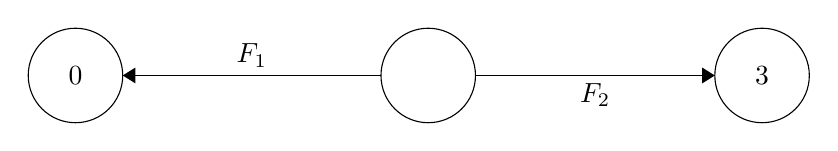
\begin{tikzpicture}[scale=0.2]
    \tikzstyle{every node}+=[inner sep=0pt]
    \draw [black] (18.7,-25.1) circle (3);
    \draw (18.7,-25.1) node {$0$};
    \draw [black] (62.3,-25.1) circle (3);
    \draw (62.3,-25.1) node {$3$};
    \draw [black] (41.1,-25.1) circle (3);
    \draw [black] (38.1,-25.1) -- (21.7,-25.1);
    \fill [black] (21.7,-25.1) -- (22.5,-25.6) -- (22.5,-24.6);
    \draw (29.9,-24.6) node [above] {$F_{1}$};
    \draw [black] (44.1,-25.1) -- (59.3,-25.1);
    \fill [black] (59.3,-25.1) -- (58.5,-24.6) -- (58.5,-25.6);
    \draw (51.7,-25.6) node [below] {$F_{2}$};
    \end{tikzpicture}
    \end{center}
\end{figure}

Si utilizamos las fórmulas calculamos el valor de $F_{1}, F_{2}$
\[
    F_{1} = \frac{1}{|0 - 1.5|} = \frac{1}{1.5}    
\]
y
\[
    F_{2} = \frac{1}{|3 - 1.5|} = \frac{1}{1.5}    
\]

Podemos ver que si restamos ambas fuerzas efectivamente el sistema está en equilibrio.

Pero ¿Qué pasa si tenemos más de dos planetas? Tenemos n - 1 soluciones ya que debemos hacer binaria entre cada pareja de planetas, si tomamos solo el planeta origen y el más alejado vamos a perder muchas soluciones.
\begin{figure}[H]
    \begin{center}
    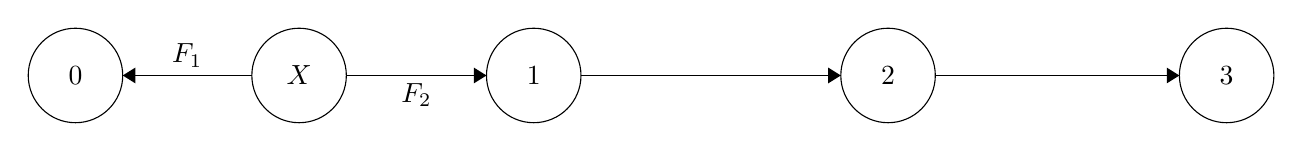
\begin{tikzpicture}[scale=0.2]
    \tikzstyle{every node}+=[inner sep=0pt]
    \draw [black] (32.4,-22.1) circle (3);
    \draw (32.4,-22.1) node {$1$};
    \draw [black] (54.9,-22.1) circle (3);
    \draw (54.9,-22.1) node {$2$};
    \draw [black] (3.3,-22.1) circle (3);
    \draw (3.3,-22.1) node {$0$};
    \draw [black] (76.4,-22.1) circle (3);
    \draw (76.4,-22.1) node {$3$};
    \draw [black] (17.5,-22.1) circle (3);
    \draw (17.5,-22.1) node {$X$};
    \draw [black] (35.4,-22.1) -- (51.9,-22.1);
    \fill [black] (51.9,-22.1) -- (51.1,-21.6) -- (51.1,-22.6);
    \draw [black] (57.9,-22.1) -- (73.4,-22.1);
    \fill [black] (73.4,-22.1) -- (72.6,-21.6) -- (72.6,-22.6);
    \draw [black] (14.5,-22.1) -- (6.3,-22.1);
    \fill [black] (6.3,-22.1) -- (7.1,-22.6) -- (7.1,-21.6);
    \draw (10.4,-21.6) node [above] {$F_{1}$};
    \draw [black] (20.5,-22.1) -- (29.4,-22.1);
    \fill [black] (29.4,-22.1) -- (28.6,-21.6) -- (28.6,-22.6);
    \draw (24.95,-22.6) node [below] {$F_{2}$};
    \end{tikzpicture}
    \end{center}
\end{figure}
Recordemos que el meteorito está en una posición válida la suma de las fuerzas debe ser igual con cero:
\[
    F_{1} + F_{2} + F_{3} + F_{3} = 0 
\]
¿Que ocurre si la suma de fuerzas no es igual con cero? Debemos de mover nuestra binaria. Si la suma es mayor que cero nos movemos a la izquierda, si es menor que cero nos movemos a la derecha.

Tomar en cuenta que si eliminas de la fórmula el valor absoluto no necesitaremos comprobar la posición del planeta en la que estamos. Si es negativo el resultado de el elemento de la fórmula que estamos haciendo entonces la fuerza que tenemos esta a la derecha en otro caso está a la izquierda.

\begin{lstlisting}
    #include <bits/stdc++.h>

    using namespace std;
    vector< double > planets;
    int n;
    //\sum^{ n }_{ 0 }{ \frac{ 1 }{ X_{i} - M } }
    double SumOfForces( double middle ){
        double sum = 0.0;
        for( int i = 0; i < n; i++ ){
            sum += 1 / ( planets[ i ] - middle );
        }
        return sum;
    }

    int main(){
        ios::sync_with_stdio( false );
        cout.tie( nullptr );
        cin.tie( nullptr );
        cin >> n;
        planets.resize( n );
        for( int i = 0; i < n; i++)
            cin >> planets[ i ];
        sort( planets.begin(), planets.end() );
        cout << n - 1 << endl; 
        for( int i = 0; i < n - 1; i++ ){
            double begin = planets[ i ];
            double end = planets[ i + 1 ];
            double middle;
            for( int i = 0; i < 25; i++ ){
                middle = ( begin + end ) / 2;
                if( SumOfForces( middle ) < 0 ){
                    begin = middle;
                } else {
                    end = middle;
                }
            }
            cout << fixed;
            cout << setprecision( 3 );
            cout << middle << " "; 
        }
        cout << endl;
        return 0;
    }
\end{lstlisting}
\chapter{Programación dinámica}
Partimos de una solución recursiva bruta y podemos hacer uso de una función de memorización. El ejemplo más clásico es el de Fibonacci
\section{Fibonacci}
\[
    fibonacci(n) = 
    \begin{cases*}
        0 & , $n = 0$ \\    
        1 & , $n = 1$ \\
        fibonacci( n - 1 ) + fibonacci( n - 2 ) & , $ n \geq 2$ 
    \end{cases*}    
\]

En código
\begin{lstlisting}
    int fibonacci( int n ){
        if( n == 0 )
            return 0;
        if( n == 1 )
            return 1;
        return fibonacci( n - 1 ) * fibonacci( n - 2 );
    }
\end{lstlisting}

Si dibujamos las llamadas recursivas como un árbol tenemos lo siguiente 

\begin{figure}[H]
    \begin{center}
        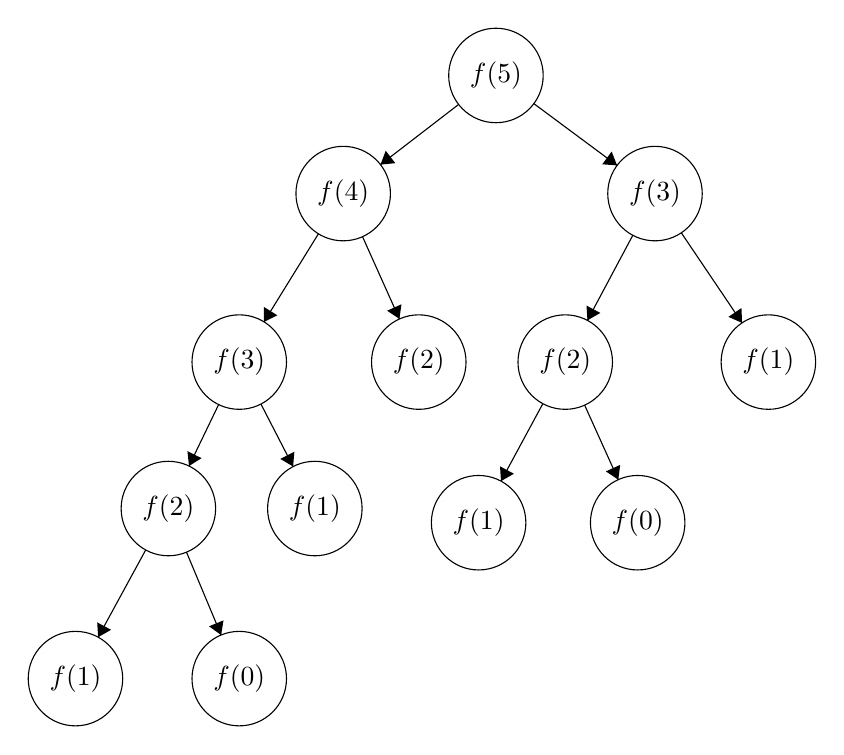
\begin{tikzpicture}[scale=0.2]
        \tikzstyle{every node}+=[inner sep=0pt]
        \draw [black] (38.5,-6.8) circle (3);
        \draw (38.5,-6.8) node {$f(5)$};
        \draw [black] (28.8,-14.3) circle (3);
        \draw (28.8,-14.3) node {$f(4)$};
        \draw [black] (48.6,-14.3) circle (3);
        \draw (48.6,-14.3) node {$f(3)$};
        \draw [black] (22.2,-25) circle (3);
        \draw (22.2,-25) node {$f(3)$};
        \draw [black] (33.6,-25) circle (3);
        \draw (33.6,-25) node {$f(2)$};
        \draw [black] (42.9,-25) circle (3);
        \draw (42.9,-25) node {$f(2)$};
        \draw [black] (55.8,-25) circle (3);
        \draw (55.8,-25) node {$f(1)$};
        \draw [black] (17.7,-34.3) circle (3);
        \draw (17.7,-34.3) node {$f(2)$};
        \draw [black] (27,-34.3) circle (3);
        \draw (27,-34.3) node {$f(1)$};
        \draw [black] (11.8,-45.1) circle (3);
        \draw (11.8,-45.1) node {$f(1)$};
        \draw [black] (22.2,-45.1) circle (3);
        \draw (22.2,-45.1) node {$f(0)$};
        \draw [black] (37.4,-35.2) circle (3);
        \draw (37.4,-35.2) node {$f(1)$};
        \draw [black] (47.5,-35.2) circle (3);
        \draw (47.5,-35.2) node {$f(0)$};
        \draw [black] (36.13,-8.64) -- (31.17,-12.46);
        \fill [black] (31.17,-12.46) -- (32.11,-12.37) -- (31.5,-11.58);
        \draw [black] (40.91,-8.59) -- (46.19,-12.51);
        \fill [black] (46.19,-12.51) -- (45.85,-11.63) -- (45.25,-12.44);
        \draw [black] (27.23,-16.85) -- (23.77,-22.45);
        \fill [black] (23.77,-22.45) -- (24.62,-22.03) -- (23.77,-21.5);
        \draw [black] (30.03,-17.04) -- (32.37,-22.26);
        \fill [black] (32.37,-22.26) -- (32.5,-21.33) -- (31.59,-21.74);
        \draw [black] (50.27,-16.79) -- (54.13,-22.51);
        \fill [black] (54.13,-22.51) -- (54.09,-21.57) -- (53.26,-22.13);
        \draw [black] (47.19,-16.95) -- (44.31,-22.35);
        \fill [black] (44.31,-22.35) -- (45.13,-21.88) -- (44.25,-21.41);
        \draw [black] (20.89,-27.7) -- (19.01,-31.6);
        \fill [black] (19.01,-31.6) -- (19.81,-31.1) -- (18.91,-30.66);
        \draw [black] (23.58,-27.67) -- (25.62,-31.63);
        \fill [black] (25.62,-31.63) -- (25.7,-30.69) -- (24.81,-31.15);
        \draw [black] (16.26,-36.93) -- (13.24,-42.47);
        \fill [black] (13.24,-42.47) -- (14.06,-42) -- (13.18,-41.53);
        \draw [black] (18.85,-37.07) -- (21.05,-42.33);
        \fill [black] (21.05,-42.33) -- (21.2,-41.4) -- (20.28,-41.78);
        \draw [black] (41.48,-27.64) -- (38.82,-32.56);
        \fill [black] (38.82,-32.56) -- (39.64,-32.09) -- (38.76,-31.62);
        \draw [black] (44.13,-27.73) -- (46.27,-32.47);
        \fill [black] (46.27,-32.47) -- (46.39,-31.53) -- (45.48,-31.94);
        \end{tikzpicture}
    \end{center}
\end{figure}

Como podemos observar hay llamadas recursivas que se repiten varias veces como ejemplo tenemos la llamada recursiva con un valor de 3, o 2. ¿Podemos evitar esto?

\begin{lstlisting}
    int memoria[ 100000 ];
    .
    .
    .
    int fibonacci( int n ){
        if( n == 0 )
            return 0;
        if( n == 1 )
            return 1;
        if( memoria[ n ] != -1 )
            return memoria[ n ];
        return memoria[ n ] = ( fibonacci( n - 1 ) * fibonacci( n - 2 ) );
    }

    int main(){
        memset( memoria, -1, sizeof(memoria) );
        .
        .
        .
    }
\end{lstlisting}

La complejidad la podemos calcular viendo los estados, en nuestro caso es el tamaño de la memoria, por ejemplo si llamamos a fibonacci de 10 siempre tenemos el mismo resultado, por tanto multiplicamos los estados por la complejidad de la función en nuestro caso es $10^{5} * constante$

\section{Coeficiente binomial}
\[
    Coef\_Bin(n, k) = 
    \begin{cases*}
        1 & , $n = k$ \\    
        1 & , $k = 0$ \\
        Coef\_Bin( n - 1, k - 1 ) + Coef\_Bin( n - 1, k ) & , $ k \leq n$ 
    \end{cases*}    
\]

Si programamos esta función tenemos lo siguiente: 

\begin{lstlisting}
    int coef_bin( int n, int k ){
        if( n == k || k == 0 )
            return 1;
        return ( coef_bin( n - 1, k - 1 ) + coef_bin( n - 1, k ) ); 
    }
\end{lstlisting}

Si aplicamos DP
\begin{lstlisting}
    memoria[ 1000 ][ 1000 ];
    .
    .
    .
    int coef_bin( int n, int k ){
        if( n == k || k == 0 )
            return 1;
        if( mem[ n ][ k ] != -1 )
            return memoria[ n ][ k ];
        return memoria[ n ][ k ] = ( coef_bin( n - 1, k - 1 ) + coef_bin( n - 1, k ) ); 
    }
\end{lstlisting}
En complejidad tenemos $O(n * k)$ y sin la función de memorización tenemos $O(2^{n})$

\section{Problema}
\textbf{Dado un grid de $n x m$, cada casilla tiene un número. Obtener un camino de la fila 1 a la fila n con suma máxima, ejemplo: }

\begin{longtable}[c]{|l|l|l|}
    \hline
    \rowcolor[HTML]{FFFFFF} 
    3                         & {\color[HTML]{333333} 5}                         & \cellcolor[HTML]{C0C0C0}{\color[HTML]{333333} 10} \\ \hline
    \endfirsthead
    %
    \endhead
    %
    \rowcolor[HTML]{FFFFFF} 
    6                         & \cellcolor[HTML]{C0C0C0}{\color[HTML]{333333} 4} & {\color[HTML]{333333} 3}                          \\ \hline
    \cellcolor[HTML]{C0C0C0}2 & 1                                                & 0                                                 \\ \hline
\end{longtable}

Como restricciones tenemos que $n, m \leq 10^{3}$ y además $A_{i,j} \leq 10^{6}$ Además solo nos podemos mover de la siguiente manera. Supongamos que estamos en el recuadro con el color gris más oscuro, estando en esa posición podemos movernos a cualquiera de los tres rectangulos con color gris más claro, es decir, podemos movernos hacía $(f + 1, c), (f + 1, c - 1), (f + 1, c + 1)$

\begin{longtable}[c]{|l|l|l|}
    \hline
    \rowcolor[HTML]{FFFFFF} 
     & \cellcolor[HTML]{656565}{\color[HTML]{333333} } & {\color[HTML]{333333} } \\ \hline
    \endfirsthead
    %
    \endhead
    %
    \rowcolor[HTML]{C0C0C0} 
     & {\color[HTML]{333333} }                         & {\color[HTML]{333333} } \\ \hline
\end{longtable}

\subsection{Solución}
\begin{lstlisting}
    int max_sum( int f, int c ){
        //Primero comprobamos si es un caso válido
        if( c < 0 || c >= m )
            return MIN_INT //MIN_INT es como un menos infinito
        //Caso base
        if( f == n )
            return grid[ f ][ c ];
        int A = max_sum( f + 1, c - 1);
        int B = max_sum( f + 1, c );
        int C = max_sum( f + 1, c + 1 );
        //No exite una función max para 3 elementos, en dado caso podemos usar vector es decir ponemos max({A, B, C})
        return max( A, max(B, C) ) + grid[ f ][ c ];
    }
\end{lstlisting}

Ahora bien ¿Cómo reducimos la complejidad de el código anterior? Debemos aplicar programación dinámica, primeramente ¿Cuál es el tamaño máximo de nuestra función de memoria? en nuestro caso es 1005 * 1005

\begin{lstlisting}
    int memoria[ 1005 ][ 1005 ];
    .
    .
    .
    int max_sum( int f, int c ){
        //Primero comprobamos si es un caso válido (que no esté fuera de rango)
        if( c < 0 || c >= m )
            return -1 //-1 es un valor bandera que identifica si ya visitamos o no la casilla
        //Caso base
        if( f == n )
            return grid[ f ][ c ];

        if( memoria[ f ][ c ] != -1 )
            return memoria[ f ][ c ]

        int A = max_sum( f + 1, c - 1);
        int B = max_sum( f + 1, c );
        int C = max_sum( f + 1, c + 1 );
        //No exite una función max para 3 elementos, en dado caso podemos usar vector es decir ponemos max({A, B, C})
        return memoria[ f ][ c ] = max( A, max(B, C) ) + grid[ f ][ c ];
    }
\end{lstlisting}

\section{Problema}
Del ejercicio anterior que sucede si podemos añadir ¿números negativos? Podemos hacer uso de otro arreglo auxiliar de booleanos, en el que marcamos si ya visitamos o no una casilla

\chapter{Problemas clásicos de DP}
\section{Mochilas}
\textbf{Vas a una tienda y quieres comprar algunos productos, digamos que hay n productos y cada producto tiene un precio y tenemos M pesos para gastar. Queremos comprar la mayor cantidad de productos gastando lo más posible.\\}
\textbf{Restricciones:}
\begin{itemize}
    \item N productos $N \leq 1000$
    \item M Pesos $M \leq 1000$
    \item $A_{i} \leq 1000$
\end{itemize}
Ejemplo:\\
N = 3, M = 8, y tenemos los productos A = {3, 4, 6} nuestro solución es comprar {3, 4} el precio es 7 y nos llevamos 4 productos.\\\\
Para poder solucionar este problema debemos de calcular el caso de probar y no probar el i-ésimo elemento. Es decir generamos todos los posibles subconjuntos del arreglo:
\begin{itemize}
    \item ()
    \item (3)
    \item (3, 4)
    \item (3, 6)
    \item (4)
    \item (4, 6)
    \item (6)
    \item (3, 4, 6)
\end{itemize}
\begin{lstlisting}
    int max_sum( int indice, int pesos_restantes ){
        //Validación, n es el número de elementos del arreglo A
        if( indice >= n )
            return 0;
        //Como no es una respuesta válida para descartarla regresamos un menos infinito
        if( pesos_restantes < 0)
            return MIN_INT;
        //Recursivamente puedo tomar o no tomar un elemento
        int tomar = max_sum( indice + 1, pesos - A[ indice ]) + A[ indice ];
        int no_tomar = max_sum( indice + 1, pesos);
        return max( tomar, no_tomar );
    }
\end{lstlisting}

Esta solución es la más bruta si queremos aplicar programación dinámica ¿Cuáles son los estados que tenemos? En este caso tendremos los índices y la cantidad de pesos restantes. Es decir:
\begin{lstlisting}
    .
    .
    .
    int memoria[ 1005 ][ 1005 ];
    bool visitado[ 1005 ][ 1005 ];
    .
    .
    .
    int max_sum( int indice, int pesos_restantes ){
        //Validación, n es el número de elementos del arreglo A
        if( indice >= n )
            return 0;
        //Como no es una respuesta válida para descartarla regresamos un menos infinito
        if( pesos_restantes < 0)
            return MIN_INT;

        if( visitado[ indice ][ pesos_restantes ] )
            return memoria[ indice ][ pesos_restantes ];
        
        //Recursivamente puedo tomar o no tomar un elemento
        int tomar = max_sum( indice + 1, pesos - A[ indice ]) + A[ indice ];
        int no_tomar = max_sum( indice + 1, pesos);
        //Como no se ha visitado el cálculo actual lo marcamos como visitado
        visitado[ indice ][ pesos_restantes ] = true;
        //Almacenamos el valor calculado en nuestra memoria
        return memoria[ indice ][ pesos_restantes ] = max( tomar, no_tomar );
    }
\end{lstlisting}

Con esta solución tenemos una complejidad de $O(n^{2})$ mientras que la solución bruta tiene una complejidad de $O(2^{n})$

\section{Mochila clásica}
\textbf{Queremos meter N piedras a una mochila cuya capacidad es de M y cada piedra tiene un valor V, queremos meter la mayor cantidad de piedras respetando que el peso límite soportado por la mochila no se exceda y se maximice el valor de las piedras dentro de la mochila\\}
\textbf{Restricciones:}
\begin{itemize}
    \item N piedras $N \leq 1000$
    \item M capacidad de la mochila $M \leq 1000$
    \item $V_{i}$ valor de la piedra $ V_{i} \leq 10^{9}$
    \item $W_{i}$ peso de la piedra $W_{i} \leq 1000$
\end{itemize}
Ejemplo:\\
N = 3, M = 50;\\
V = [ 60, 100, 120 ]\\
W = [ 10, 20, 30 ]\\
Para este caso tenemos como solución tomar la segunda y tercer piedra teniendo un valor de 220 y un peso de 50, el cual puede soportar perfectamente nuestra mochila.\\

Podemos encontrar una solución siguiendo más o menos lo mismo que el ejercico anterior, vamos a tratar de maximizar el valor tomando o no tomando el i-ésimo peso 

\begin{lstlisting}
    int sum_max( int indice, int capacidad ){
        if( indice >= n )
            return 0;
        if( capacidad < 0 )
            return MIN_INT;
        //Si lo tomo cuál es el valor máximo que podemos tener con la respuesta actual?
        int tomar = sum_max( indice + 1, capacidad - W[ indice ] ) + V[ indice ];
        int no_tomar = sum_max( indice + 1, capacidad );
        return max(tomar, no_tomar);
    }
\end{lstlisting}

Si aplicamos programación dinámica
\begin{lstlisting}
    .
    .
    .
    int memoria[ 1005 ][ 1005 ];
    .
    .
    .
    int sum_max( int indice, int capacidad ){
        if( indice >= n )
            return 0;
        if( capacidad < 0 )
            return MIN_INT;
        if( memoria[ indice ][ capacidad ] != MIN_INT )
            return memoria[ indice ][ capacidad ];
        //Si lo tomo cuál es el valor máximo que podemos tener con la respuesta actual?
        int tomar = sum_max( indice + 1, capacidad - W[ indice ] ) + V[ indice ];
        int no_tomar = sum_max( indice + 1, capacidad );
        return memoria[ indice ][ capacidad ] = max(tomar, no_tomar);
    }
\end{lstlisting}

Ahora bien debemos responder ¿dónde está la respuesta a nuestro problema?

\begin{lstlisting}
    .
    .
    .
    int main(){
        .
        .
        .
        //Si indexamos desde cero aquí estará la solución
        cout << sum_max( 0, M );
        .
        .
        .
        return 0;
    }
\end{lstlisting}

\section{Problema}
\textbf{Imagina que compraste algo en algúna tienda, supermercado, etc, tienes que pagar con N monedas, pero quieres saber ¿De cuantas formas utilizando cualquiera de esas N monedas puedo dar el cambio (M)?\\}
\textbf{Restricciones: }
\begin{itemize}
    \item N monedas $N \leq 1000$
    \item M cambio $N \leq 1000$
    \item $C_{i}$ Monedas $1 leq C_{i} \leq 1000$
\end{itemize}
Ejemplo:
N = 4, M = 5\\
C = [ 1, 2, 3, 4 ] //Indexado desde cero \\
\begin{itemize}
    \item { (0, 3) = 1 + 4 = 5 }
    \item { (1, 2) = 2 + 3 = 5 }
\end{itemize}

Es decir nuevamente debemos de considerar el problema como tomar o no tomar

\begin{figure}[H]
    
\begin{center}
    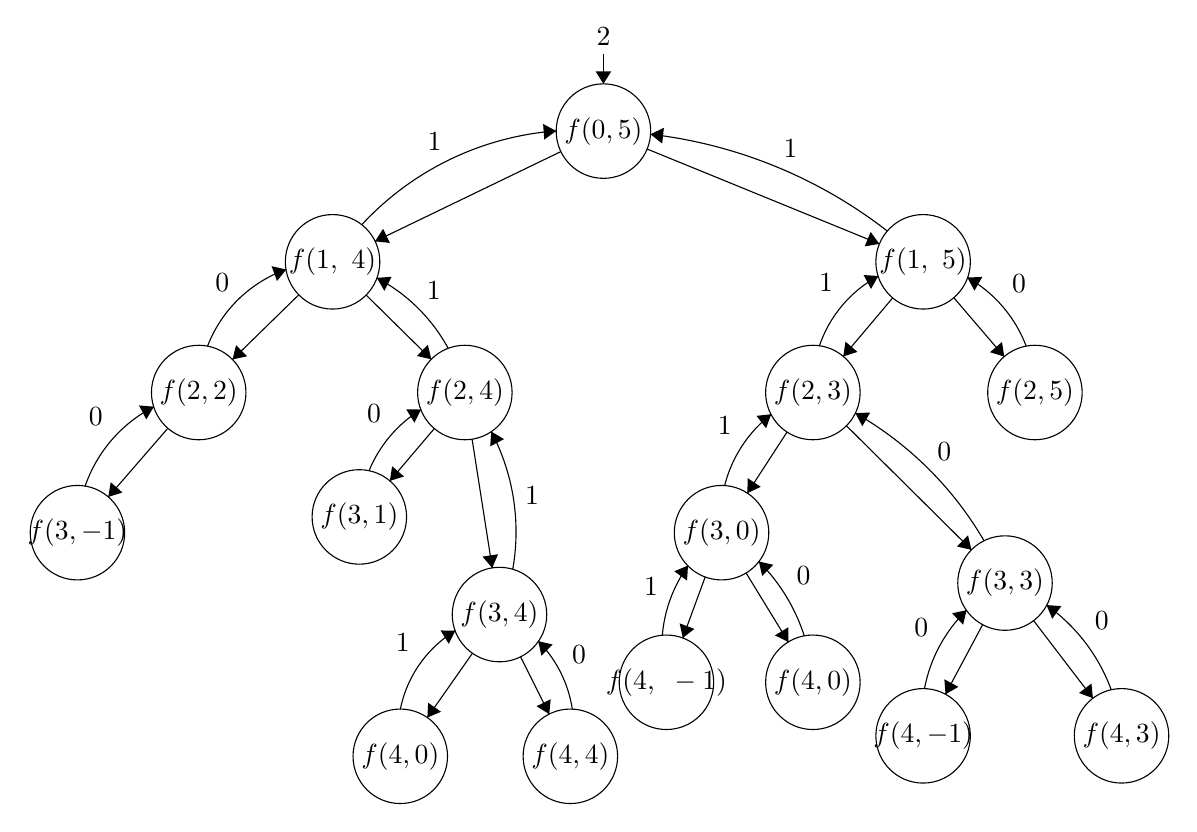
\begin{tikzpicture}[scale=0.2]
    \tikzstyle{every node}+=[inner sep=0pt]
    \draw [black] (38.5,-6.8) circle (3);
    \draw (38.5,-6.8) node {$f(0,5)$};
    \draw [black] (21.3,-15.1) circle (3);
    \draw (21.3,-15.1) node {$f(1,\mbox{ }4)$};
    \draw [black] (58.8,-15.1) circle (3);
    \draw (58.8,-15.1) node {$f(1,\mbox{ }5)$};
    \draw [black] (12.8,-23.4) circle (3);
    \draw (12.8,-23.4) node {$f(2,2)$};
    \draw [black] (29.7,-23.4) circle (3);
    \draw (29.7,-23.4) node {$f(2,4)$};
    \draw [black] (5.1,-32.3) circle (3);
    \draw (5.1,-32.3) node {$f(3,-1)$};
    \draw [black] (51.8,-23.4) circle (3);
    \draw (51.8,-23.4) node {$f(2,3)$};
    \draw [black] (65.9,-23.4) circle (3);
    \draw (65.9,-23.4) node {$f(2,5)$};
    \draw [black] (23,-31.3) circle (3);
    \draw (23,-31.3) node {$f(3,1)$};
    \draw [black] (31.9,-37.5) circle (3);
    \draw (31.9,-37.5) node {$f(3,4)$};
    \draw [black] (25.6,-46.5) circle (3);
    \draw (25.6,-46.5) node {$f(4,0)$};
    \draw [black] (36.4,-46.5) circle (3);
    \draw (36.4,-46.5) node {$f(4,4)$};
    \draw [black] (46,-32.3) circle (3);
    \draw (46,-32.3) node {$f(3,0)$};
    \draw [black] (64,-35.5) circle (3);
    \draw (64,-35.5) node {$f(3,3)$};
    \draw [black] (58.8,-45.2) circle (3);
    \draw (58.8,-45.2) node {$f(4,-1)$};
    \draw [black] (71.4,-45.2) circle (3);
    \draw (71.4,-45.2) node {$f(4,3)$};
    \draw [black] (42.5,-41.8) circle (3);
    \draw (42.5,-41.8) node {$f(4,\mbox{ }-1)$};
    \draw [black] (51.8,-41.8) circle (3);
    \draw (51.8,-41.8) node {$f(4,0)$};
    \draw [black] (35.8,-8.1) -- (24,-13.8);
    \fill [black] (24,-13.8) -- (24.94,-13.9) -- (24.51,-13);
    \draw [black] (41.28,-7.94) -- (56.02,-13.96);
    \fill [black] (56.02,-13.96) -- (55.47,-13.2) -- (55.09,-14.12);
    \draw [black] (19.15,-17.2) -- (14.95,-21.3);
    \fill [black] (14.95,-21.3) -- (15.87,-21.1) -- (15.17,-20.39);
    \draw [black] (23.43,-17.21) -- (27.57,-21.29);
    \fill [black] (27.57,-21.29) -- (27.35,-20.37) -- (26.65,-21.08);
    \draw [black] (10.84,-25.67) -- (7.06,-30.03);
    \fill [black] (7.06,-30.03) -- (7.96,-29.75) -- (7.21,-29.1);
    \draw [black] (56.87,-17.39) -- (53.73,-21.11);
    \fill [black] (53.73,-21.11) -- (54.63,-20.82) -- (53.87,-20.17);
    \draw [black] (60.75,-17.38) -- (63.95,-21.12);
    \fill [black] (63.95,-21.12) -- (63.81,-20.19) -- (63.05,-20.84);
    \draw [black] (27.76,-25.69) -- (24.94,-29.01);
    \fill [black] (24.94,-29.01) -- (25.84,-28.73) -- (25.08,-28.08);
    \draw [black] (30.16,-26.36) -- (31.44,-34.54);
    \fill [black] (31.44,-34.54) -- (31.81,-33.67) -- (30.82,-33.82);
    \draw [black] (30.18,-39.96) -- (27.32,-44.04);
    \fill [black] (27.32,-44.04) -- (28.19,-43.67) -- (27.37,-43.1);
    \draw [black] (33.24,-40.18) -- (35.06,-43.82);
    \fill [black] (35.06,-43.82) -- (35.15,-42.88) -- (34.25,-43.32);
    \draw [black] (50.16,-25.91) -- (47.64,-29.79);
    \fill [black] (47.64,-29.79) -- (48.49,-29.39) -- (47.66,-28.84);
    \draw [black] (53.93,-25.51) -- (61.87,-33.39);
    \fill [black] (61.87,-33.39) -- (61.65,-32.47) -- (60.95,-33.18);
    \draw [black] (62.58,-38.14) -- (60.22,-42.56);
    \fill [black] (60.22,-42.56) -- (61.04,-42.09) -- (60.15,-41.61);
    \draw [black] (65.82,-37.89) -- (69.58,-42.81);
    \fill [black] (69.58,-42.81) -- (69.49,-41.88) -- (68.7,-42.48);
    \draw [black] (23.154,-12.745) arc (137.20989:94.31013:18.749);
    \fill [black] (35.5,-6.79) -- (34.67,-6.35) -- (34.74,-7.34);
    \draw (27.78,-8.09) node [above] {$1$};
    \draw [black] (13.355,-20.468) arc (159.00785:109.62803:8.366);
    \fill [black] (18.36,-15.59) -- (17.43,-15.38) -- (17.77,-16.32);
    \draw (14.3,-17) node [above] {$0$};
    \draw [black] (5.585,-29.354) arc (-198.95042:-242.78023:8.946);
    \fill [black] (9.95,-24.3) -- (9.01,-24.22) -- (9.47,-25.11);
    \draw (6.74,-24.96) node [left] {$0$};
    \draw [black] (24.111,-16.121) arc (62.21244:28.47373:10.983);
    \fill [black] (24.11,-16.12) -- (24.59,-16.94) -- (25.05,-16.05);
    \draw (27.73,-17.55) node [above] {$1$};
    \draw [black] (23.611,-28.38) arc (157.76368:121.63368:8.246);
    \fill [black] (26.92,-24.48) -- (25.98,-24.47) -- (26.5,-25.32);
    \draw (24.41,-24.72) node [left] {$0$};
    \draw [black] (31.377,-25.88) arc (27.76697:-10.03044:13.665);
    \fill [black] (31.38,-25.88) -- (31.31,-26.82) -- (32.19,-26.36);
    \draw (33.49,-29.94) node [right] {$1$};
    \draw [black] (25.601,-43.519) arc (-191.3248:-238.65924:7.6);
    \fill [black] (29.1,-38.52) -- (28.16,-38.51) -- (28.68,-39.36);
    \draw (26.23,-39.29) node [left] {$1$};
    \draw [black] (34.359,-39.186) arc (44.59265:8.53745:7.831);
    \fill [black] (34.36,-39.19) -- (34.56,-40.11) -- (35.28,-39.4);
    \draw (36.48,-40.07) node [right] {$0$};
    \draw [black] (46.194,-29.323) arc (-194.05678:-232.12662:8.313);
    \fill [black] (49.15,-24.78) -- (48.22,-24.88) -- (48.83,-25.67);
    \draw (46.68,-25.48) node [left] {$1$};
    \draw [black] (52.21,-20.446) arc (-198.71388:-241.57291:7.955);
    \fill [black] (55.96,-16) -- (55.02,-15.94) -- (55.49,-16.82);
    \draw (53.11,-16.43) node [left] {$1$};
    \draw [black] (61.613,-16.096) arc (60.36187:20.72692:8.481);
    \fill [black] (61.61,-16.1) -- (62.06,-16.93) -- (62.56,-16.06);
    \draw (64.41,-16.51) node [right] {$0$};
    \draw [black] (54.497,-24.708) arc (60.25935:30.21222:22.202);
    \fill [black] (54.5,-24.71) -- (54.94,-25.54) -- (55.44,-24.67);
    \draw (60.14,-27.74) node [above] {$0$};
    \draw [black] (58.883,-42.214) arc (-190.71414:-225.67582:9.427);
    \fill [black] (61.56,-37.22) -- (60.64,-37.42) -- (61.34,-38.14);
    \draw (59.16,-38.34) node [left] {$0$};
    \draw [black] (66.643,-36.902) arc (54.54567:20.13338:11.436);
    \fill [black] (66.64,-36.9) -- (67,-37.77) -- (67.58,-36.96);
    \draw (69.67,-37.88) node [right] {$0$};
    \draw [black] (41.492,-6.999) arc (83.35606:52.16787:30.209);
    \fill [black] (41.49,-7) -- (42.23,-7.59) -- (42.34,-6.59);
    \draw (50.39,-8.53) node [above] {$1$};
    \draw [black] (44.96,-35.12) -- (43.54,-38.98);
    \fill [black] (43.54,-38.98) -- (44.28,-38.41) -- (43.34,-38.06);
    \draw [black] (47.56,-34.86) -- (50.24,-39.24);
    \fill [black] (50.24,-39.24) -- (50.25,-38.3) -- (49.39,-38.82);
    \draw [black] (42.239,-38.826) arc (-184.72078:-215.72893:8.834);
    \fill [black] (43.87,-34.39) -- (43,-34.75) -- (43.81,-35.34);
    \draw (42,-35.7) node [left] {$1$};
    \draw [black] (48.368,-34.129) arc (45.01101:17.79931:11.777);
    \fill [black] (48.37,-34.13) -- (48.58,-35.05) -- (49.29,-34.34);
    \draw (50.73,-35.05) node [right] {$0$};
    \draw [black] (38.5,-1.9) -- (38.5,-3.8);
    \draw (38.5,-1.4) node [above] {$2$};
    \fill [black] (38.5,-3.8) -- (39,-3) -- (38,-3);
    \end{tikzpicture}
    \end{center}
\end{figure}

Como solución bruta ¿Qué podemos programar?
\begin{lstlisting}
    .
    .
    .
    int cuenta( int indice, int cambio ){
        //Verificamos que no nos salgamos del rango
        if( indice == n ){
            //Si llegamos al límite verificamos si lo que tenemos es una solución válida
            if( cambio == 0 )
                //Como encontramos una solución la contamos
                return 1;
            //Como no hay solución retornamos cero
            return 0;
        }
        //Si el cambio es negativo no es una combinación válida
        if( cambio < 0 )
            return 0;
        //Intentamos tomando el elemento actual
        int tomar = cuenta( indice + 1, cambio - C[ indice ] );
        int no_tomar = cuenta( indice + 1, cambio );
        return tomar + no_tomar;
    }
\end{lstlisting}

Si añadimos programación dinámica tenemos lo siguiente

\begin{lstlisting}
    .
    .
    .
    int memoria[ 1005 ][ 1005 ];
    bool visitado[ 1005 ][ 1005 ];
    .
    .
    .
    int cuenta( int indice, int cambio ){
        //Verificamos que no nos salgamos del rango
        if( indice == n ){
            //Si llegamos al límite verificamos si lo que tenemos es una solución válida
            if( cambio == 0 )
                //Como encontramos una solución la contamos
                return 1;
            //Como no hay solución retornamos cero
            return 0;
        }
        //Si el cambio es negativo no es una combinación válida
        if( cambio < 0 )
            return 0;
    
        if( visitado[ indice ][ cambio ] )
            return memoria[ indice ][ cambio ];
        //Intentamos tomando el elemento actual
        int tomar = cuenta( indice + 1, cambio - C[ indice ] );
        int no_tomar = cuenta( indice + 1, cambio );
        visitado[ indice ][ cambio ] = true;
        return memoria[ indice ][ cambio ] = (tomar + no_tomar);
    }
\end{lstlisting}


\section{Boredrom}
\textbf{Vamos a tomar el $a_{k}$ elemento, vamos remover de nuestro arrego el $a_{k} + 1$ y $a_{k} - 1$ }\\
\textbf{Restricciones: }
1 1 2 2 2 2 2 3 3 \\
En este caso elegimos el 2 y removemos los unos y los tres nos queda \\
2 2 2 2 2 \\ 
Como no tenemos más elementos para elegir nuestra respuesta es la suma de los elementos restantes es decir 5 \\
¿Cómo podemos programar eso?
\begin{lstlisting}
    #include <bits/stdc++.h>

    using namespace std;
    typedef long long int lli;
    lli bucket[ 100005 ];
    lli DP[ 100005 ];
    bool visited[ 100005 ];
    lli n;
    int MAX = -1;
    
    lli max_sum( int index ){
    
        if( index >= MAX + 1)
            return 0;
        
        if( visited[ index ] )
            return DP[ index ];
        visited[ index ] = true;
        //Tomamos el elemento actual
        lli take = max_sum( index + 2 ) + ( bucket[ index ] * index );
        //Nos saltamos el elemento actual
        lli not_take = max_sum( index + 1 );
    
        return DP[ index ] = max( take, not_take );
    }
    
    int main(){
        cin >> n;
        for( int i = 0, v; i < n; i++){
            cin >> v;
            MAX = max( MAX, v );
            //Generamos nuestra cubeta
            bucket[ v ]++;
        }
        
        cout << max_sum( 1 ) << endl;
        return 0;
    }
\end{lstlisting}